%!TEX root = /Users/louis/Documents/PhD/Deliverables/Thesis/thesis.tex

\section{MDE Tools}
\label{sec:mde_tools}
For model-driven engineering to be applicable in the large, and to complex systems, mature and powerful tools and languages must be available. Such tools and languages are beginning to emerge, and this section discusses the state of current MDE development environments, which are typically a combination of tools and languages.

% e.g., model-to-
% model (M2M) transformation tools such as ATL \cite{atl} and VIATRA \cite{viatra}, workflow architectures such as oAW \cite{oaw}, and model-to-text (M2T) transformation tools such as MOFScript \cite{oldevik05toward} and XPand \cite{xpand}.

This section provides a brief overview of the Eclipse Modelling Framework \cite{emf}, which underpins many of MDE tools and languages, facilitating their interoperability. Subsequently, a discussion of Epsilon \cite{epsilon}, an extensible platform for the specification of model management languages, is presented. The highly extensible nature of Epsilon (which is described below) makes it an ideal host for the rapid prototyping of languages and exploring research hypotheses.  

\subsection{Eclipse Modelling Framework}
\label{subsec:emf}
\cite{eclipse} is an open-source community whose projects seek to build an extensible development platform. The Eclipse Modelling Framework (EMF) project \cite{emf} enables MDE within Eclipse. EMF provides a modelling framework with code generation facilities, and a meta-modelling language, Ecore, that implements the MOF 2.0 specification \cite{mof}. EMF is arguably the most widely-used contemporary MDE modelling framework.

EMF provide metamodel-specific editors for loading, storing and constructing models. EMF model editors comprise a navigation view that depicts the model as a structure and a properties view that is used to specify the values of model element features. By default, EMF editors represent models on disk as XMI 2.1 \cite{xmi} documents.  Figure~\ref{fig:emf_model_editor} shows an EMF model editor for a simplistic state machine language. 

\begin{figure}[htbp]
  \begin{center}
    \leavevmode
    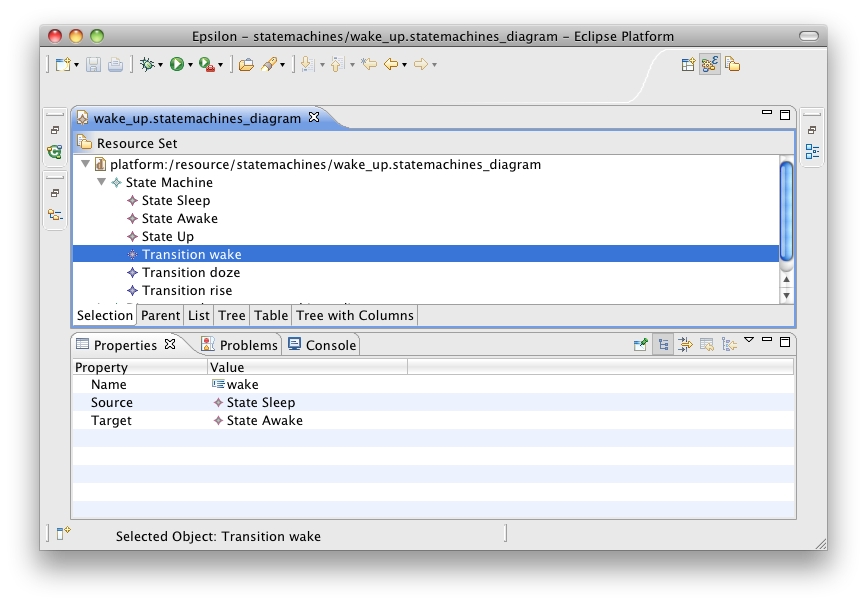
\includegraphics[width=10cm]{2.Background/images/emf_model_editor.png}
  \end{center}
  \caption{EMF state machine model editor.}
  \label{fig:emf_model_editor}
\end{figure}

Users of EMF can define their own metamodels in Ecore and generate a corresponding model editor. EMF provides both a tree-based editor (Figure~\ref{fig:emf_metamodel_editor_tree}) and a diagrammatic editor (Figure~\ref{fig:emf_metamodel_editor_diagrammatic}) for constructing metamodels. The latter uses syntax taken from UML class diagrams. An extension to EMF provides a textual editor for metamodels (Figure~\ref{fig:emf_metamodel_editor_textual}).


\begin{figure}[htbp]
  \begin{center}
    \leavevmode
    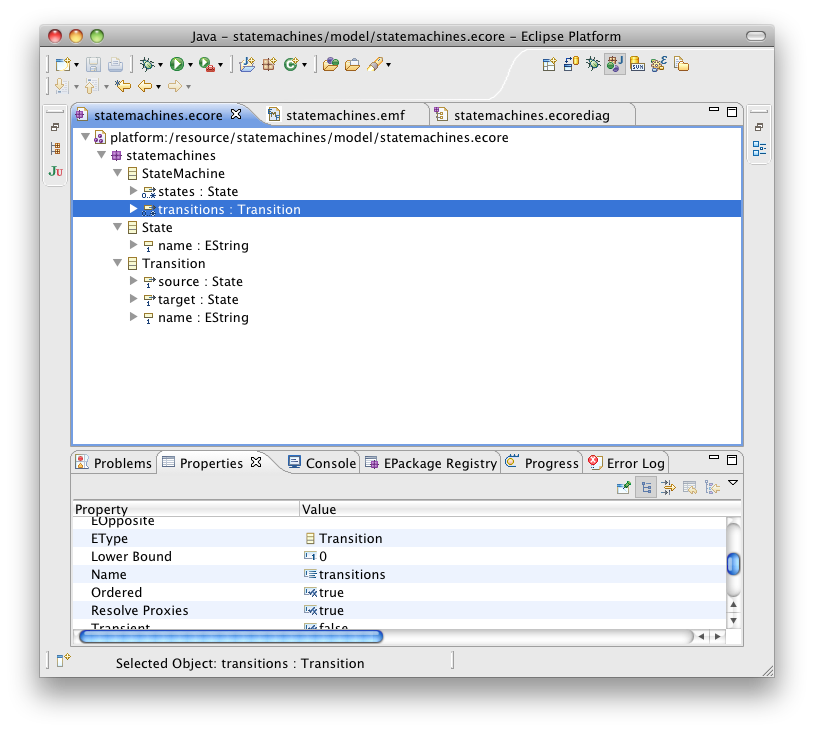
\includegraphics[width=10cm]{2.Background/images/emf_metamodel_tree.png}
  \end{center}
  \caption{EMF tree-based metamodel editor.}
  \label{fig:emf_metamodel_editor_tree}
\end{figure}

\begin{figure}[htbp]
  \begin{center}
    \leavevmode
    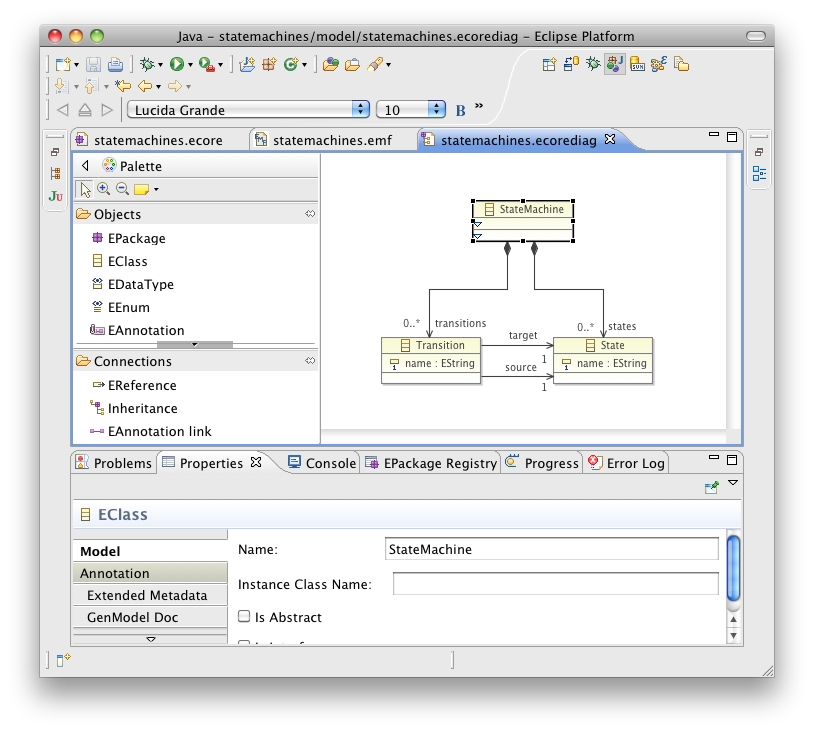
\includegraphics[width=10cm]{2.Background/images/emf_metamodel_diagrammatic.png}
  \end{center}
  \caption{EMF diagrammatic metamodel editor.}
  \label{fig:emf_metamodel_editor_diagrammatic}
\end{figure}

\begin{figure}[htbp]
  \begin{center}
    \leavevmode
    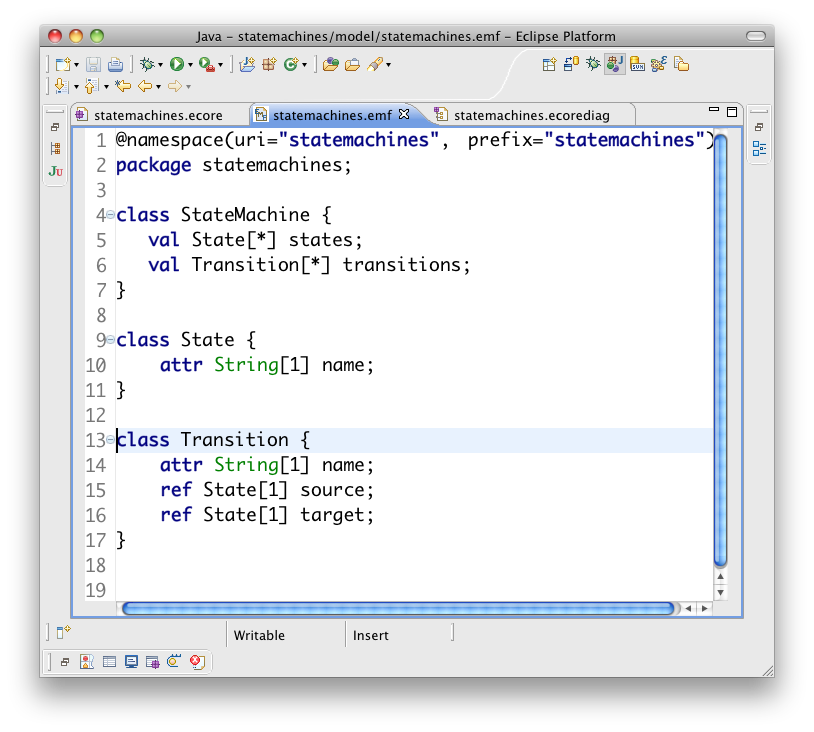
\includegraphics[width=10cm]{2.Background/images/emf_metamodel_textual.png}
  \end{center}
  \caption{EMF textual metamodel editor.}
  \label{fig:emf_metamodel_editor_textual}
\end{figure}

The range of concrete syntaxes for Ecore models presents a challenge for tools that wish to augment the way in which metamodels are defined (e.g. for specifying semantics). Extensions made to one type of metamodel editor (e.g. tree-based) will not be automatically be available in others (e.g. visual and textual). However, EMF does facilitate the programmatic monitoring of model changes, which can be used for implementing metamodel extensions, as discussed in Chapter~\ref{Implementation}. 

From an Ecore model, EMF can generate a metamodel-specific model editor. The metamodel specified in Figure~\ref{fig:emf_metamodel_editor} was used to generate the Java code for the model editor shown in Figure~\ref{fig:emf_model_editor}. Because model editors are generated from metamodels, models and metamodels are kept separate in EMF. Consequently, metamodel changes cannot be propagated directly to models.

The Graphical Modeling Framework (GMF) \cite{gronback09emp} is used to specify graphical concrete syntax for metamodels defined in EMF. GMF itself uses a model-driven approach: users specify several models, which are combined, transformed and then used to generate code for the resulting graphical editor. Figure~\ref{fig:gmf_model_editor} shows a model editor produced with GMF for the simplistic state machine language described above.

\begin{figure}[htbp]
  \begin{center}
    \leavevmode
    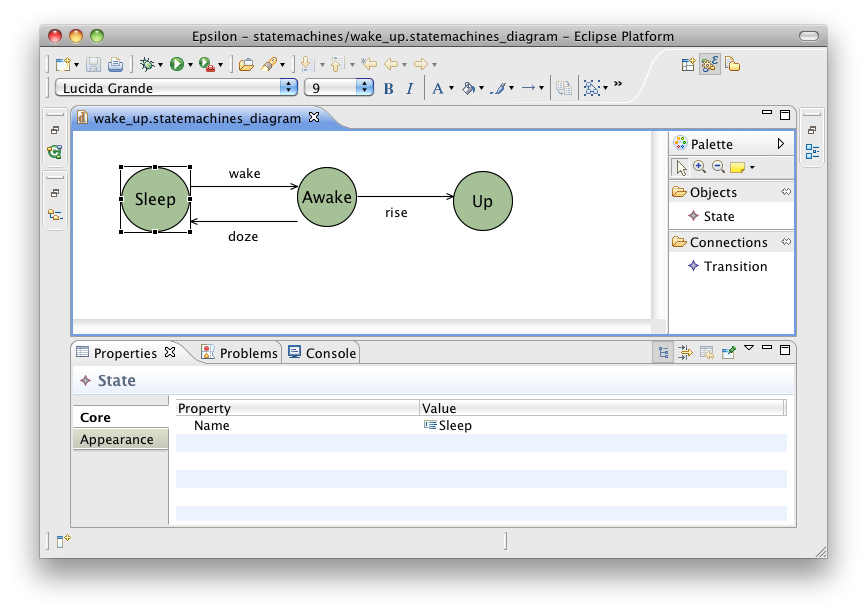
\includegraphics[width=10cm]{2.Background/images/gmf_model_editor.png}
  \end{center}
  \caption{GMF state machine model editor.}
  \label{fig:gmf_model_editor}
\end{figure}

Many MDE tools are interoperable with EMF, enriching its functionality. The remainder of this section discusses one tool that is interoperable with EMF, Epsilon, which is a suitable platform for rapid prototyping of model management languages and, hence, is useful for performing MDE research.

\subsection{Epsilon}
\label{subsec:epsilon}
The Extensible Platform for Specification of Integrated Languages for mOdel maNagement (Epsilon) \cite{epsilon} is a suite of tools and domain-specific languages for MDE. Epsilon comprises several integrated model management languages -- built atop a common infrastructure -- for performing tasks such as model merging, model transformation and inter-model consistency checking \cite{kolovos09thesis}. 

Figure \ref{fig:epsilon} illustrates the various components of Epsilon.

Whilst many model management languages are bound to a particular subset of modelling technologies, limiting their applicability, Epsilon is metamodel-agnostic -- models written in any modelling language can be manipulated by Epsilon's model management languages \cite{kolovos06eol}. Currently, Epsilon supports models implemented using EMF, MOF 1.4, XML, or Community Z Tools (CZT) \footnote{\url{http://czt.sourceforge.net/}}. Interoperability with further modelling technologies can be achieved via extensions of the Epsilon Model Connectivity (EMC) layer. 

\begin{figure}[htbp]
  \begin{center}
    \leavevmode
    \includegraphics[scale=0.6]{Epsilon.png}
  \end{center}
  \caption{The architecture of Epsilon, taken from \cite{rose08egl}.}
  \label{fig:epsilon}
\end{figure}

The architecture of Epsilon promotes reuse when building task-specific model management languages and tools.  Each Epsilon language can be reused wholesale in the production of new languages. Ideally, the developer of a new language only has to design language concepts and logic that do not already exist in Epsilon languages. As such, new task-specific languages can be implemented in a minimalistic fashion. This claim has been demonstrated in \cite{rose08egl}, which describes the Epsilon Generation Language (EGL) for specifying model-to-text transformation.

The core language, the Epsilon Object Language (EOL) \cite{kolovos06eol}, provides functionality similar to that of OCL \cite{ocl2}. However, EOL provides an extended feature set, which includes the ability to update models, access to multiple models, conditional and loop statements, statement sequencing, and provision of standard output and error streams.

As shown in Figure \ref{fig:epsilon}, every Epsilon language re-uses EOL, so improvements to this language enhance the entire platform. EOL also allows developers to delegate computationally intensive tasks to extension points, where the task can be authored in Java.

Epsilon is a member of the Eclipse GMT \cite{gmt} project, a research incubator for the top-level modelling technology project. Epsilon provides a lightweight means for defining new experimental languages for MDE. For these reasons, Epsilon is uniquely positioned as an ideal host for the rapid prototyping of languages for model management.